\chapter{Risk Analysis}
	The Risk Analysis table defines a potential set of risks that our group could face, as setbacks to timely progression towards our finished project. For each risk, there are two potential consequences, a probability value (0$\rightarrow$1), a severity value (0$\rightarrow$10), an impact value (impact=probability*severity), and two potential mitigation strategies. The risks are ordered from greatest to least impact value (top-to-bottom).

\begin{table}[]
\caption{Risk Table}
\label{riskTable}
\begin{tabular}{l}
    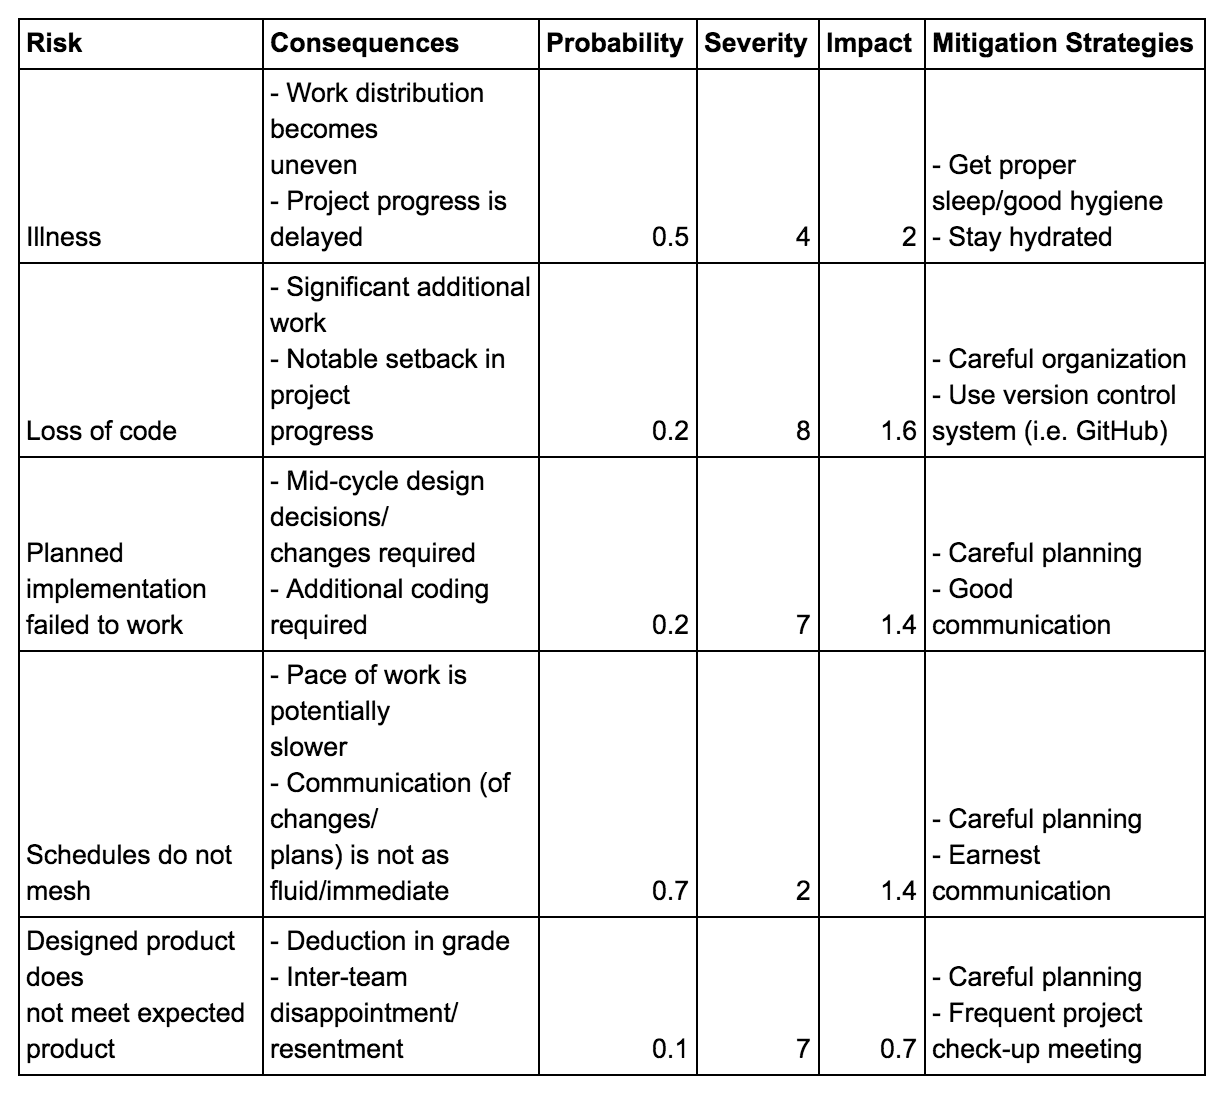
\includegraphics[scale = 0.5]{riskTable.png}
\end{tabular}
\end{table}

\chapter{Sustainability}
	Sustainability is an essential factor in delivering a product that will benefit people’s lives and create value. During the design of PRAHVI, we have identified multiple points of sustainability through the lifecycle of the product: from its environmental costs, to its user interaction, and its economic viability. By evaluating these facets, we can draw a concrete “triple bottom line” to evaluate the effectiveness of the product in the context of an actual business model.
	
	As a product, PRAHVI is designed primarily using off-the-shelf components that have been developed at scale both to reduce costs and to minimize its environmental footprint. Its construction consists mainly of a PCB board, a camera module, a plastic enclosure, and a cable to connect the product to the user’s smartphone. The board used in the current version is known as a Raspberry Pi Zero, a lightweight, low-power board designed for mobile applications. This means that PRAHVI operates using less than 100mW and can be powered entirely by a smartphone’s accessory port. The electrical components are manufactured in compliance with the global Restriction of the Use of certain Hazardous Substances (RoHS) regulation. Additionally, each company we have sourced components from have publicly pledged their products to be free of conflict materials and use minimal amounts of rare-earth metals. This allows us to minimize the environmental impact of both construction and disposal of the product by accounting for its individual materials and following federal and international procedures. The enclosure is constructed using a 3D printer with ABS plastic material. Although this material is not biodegradable, using a pure ABS filament and designing the product to be modular allows a recycling entity to separate the components and recycle the ABS plastic. Overall, we anticipate a single PRAHVI unit to last the life cycle of the user’s smartphone, typically 2-3 years. This accounts for future feature upgrades and the general durability of the product against normal wear and tear. By accounting for each of these factors during the design phase of our project, we can minimize PRAHVI’s overall environmental footprint.
	
	In terms of social sustainability, we have chosen a very clear demographic that has been largely untapped for innovation making PRAHVI a promising product for this field. PRAHVI is designed to assist users with visual disabilities navigate their visually-oriented environments, from casual reading to discovering signs and posters. The use cases it presents are context-specific but very familiar to those who struggle with these tasks on a daily basis. Because we are tailoring the interface of the product to individuals with partial or full visual disability, making the product intuitive presents a unique challenge for us. By crafting an interface that communicates primarily through sound and haptic feedback, we believe that the product will be intuitive and useful for the user. Furthermore, we hope to begin testing the product through usage exercises and potentially real-world user tests. However, creating a product for this niche also draws the factor that users will create an implicit dependence on the product. Should the user begin entering high-risk environments on their own, such as navigating a busy street, the stakes for failure could mean the difference between life or death. Therefore, for the first few iterations of the product, we would advise users only to use the product in a controlled environment with minimal hazards and many safeguards. Overall, we hope that PRAHVI can add significant value to a user’s daily life with the objectives we have set, using the technologies and sense of interface we have developed.
	
	The final metric for a product’s viability involves the economic sustainability, particularly in a world saturated with electronic assistance devices. By utilizing off-the-shelf components and relying on a smartphone that users in this demographic typically already have, we have made strides in minimizing the cost of the product to well below current solutions. Our target cost of the product is to be less than \$200, which is a fraction of the closest competing product, OrCam, which is priced at \$2500. Much of the cost for such devices is in the software and the processing unit, as these devices are typically designed to be standalone. During the design phase of our project, we studied the demographic of individuals with visual disabilities and found that many typically own and use a smartphone on a daily basis. This means that we can safely trade off a small measure of convenience with a standalone device for the cost savings of using a processing unit users already own. Additionally, this drives down the cost and frequency of future upgrades, as the device’s processing power is upgraded for free with every new smartphone a user purchases. This means less revenue is spent on developing and manufacturing new PRAHVI processing modules. As a product, most of the revenue would go to the material cost of the components and development and testing of the software. Additionally, the retail cost to the end user can typically be augmented by support from their insurance providers. In the future, PRAHVI may be manufactured entirely using a custom PCB board and custom hardware that, manufactured at scale, would further drive down costs while delivering a more integrated product. From an economic standpoint, PRAHVI is an effective product in this segment, especially compared to competing products, by using a careful mix of tradeoffs that overall benefit users.
	
	As a product, we hope that PRAHVI meets or exceeds the “triple bottom line” to remain a fully-sustainable product. By identifying a key niche ripe for innovation, then sourcing parts and development in an environmentally and economically responsible way, we envision a life cycle that helps the product remain viable for many iterations. With each iteration, we also hope that the product can execute fixes and improvements that make it more useful for users and even expand its target audience. These goals overall help create the framework for a transition from a simple design project into an actual product.
	
	In a world with increasingly limited natural resources and a larger focus on industrial impact on our environment, sustainability is a significant part of research and development. During the design of PRAHVI, we have identified processes, components, and the sourcing of these components to evaluate its environmental impact. As a product that spans the resources of multiple industries, we recognize that our product’s lifecycle includes many stakeholders and resources, from manufacture, to daily usage, and final disposal.
	
	The construction of PRAHVI begins with its components, their sourcing, and overall assembly. The primary component of the device is its printed circuit board (PCB). For research purposes, we have used an off-the-shelf board known as the Raspberry Pi Zero. This board consists of plastic for the board itself, laser-etched copper traces, and components with varying amounts of copper, silicon, and gold. In compliance with the global Restriction of the Use of Certain Hazardous Substances (RoHS) regulation, the Raspberry Pi is manufactured without the use of conflict materials and minimal use of rare-earth elements. In addition, the camera module manufactured by Sony Inc. is manufactured under stricter regulations that replace many materials, such as those that go into the imaging sensor, with more environmentally-friendly, albeit slightly more expensive alternatives. We found that the small form factor of the Raspberry Pi not only makes the product more portable, but holistically uses fewer materials to manufacture, further driven down by the large scale of the Raspberry Pi, while still meeting our quality and performance requirements. Although other boards and modules were evaluated, most are manufactured under small-scale operations that use more resources or did not meet our requirements. The case of the product is manufactured using a 3D printer with ABS plastic material. This material is not biodegradable, and must be recycled at the end of the product’s lifecycle. During the design phase of this project, we selected what we believe are the optimal components and materials for PRAHVI from a performance and environmental standpoint.
	
	As a holistic product, PRAHVI introduces challenges to managing energy consumption from manufacture, to delivery, and daily use. The parts used in PRAHVI are sourced primarily from China. With careful design and planning, we consolidated our parts orders into three stages and from a single supplier to ensure that we minimized the impact of transportation in the product. The case, which is manufactured using a MakerBot Replicator 2X, is the only part we manufacture ourselves. For research purposes, using a 3D printer significantly reduces the energy and resource overhead of a professional manufacturer, while providing a representative component of the final product. During use, we anticipate that PRAHVI will be powered entirely using a smartphone device, removing the need for a separate battery. Its small form-factor and ARM processor allows PRAHVI to operate with minimal power use. We further these energy savings by defining clear contexts in which PRAHVI is in a passive “sleep” mode and when it is in an active “scanning” mode. These practices combined help to minimize the overall energy footprint of PRAHVI as a product.
	
	Finally, although PRAHVI is designed with longevity of the product in-mind, we incorporated its transition out into the design process. PRAHVI is made with standard components, each of which can be easily replaced. We anticipate that PRAHVI can be used throughout the standard lifecycle of a smartphone, around two years. This accounts for component failures, the likelihood of damage resulting in a system failure, and required feature upgrades for new versions of the smartphone’s software. At the end of the device’s lifecycle, the components of the Raspberry Pi Zero can be easily extracted and recycled through standard protocols. In addition, the case is entirely constructed from ABS plastic that can also be recycled and repurposed. These considerations help ensure that PRAHVI is built to last with the user’s needs as well as transition out of use in a sustainable manner.

\chapter{Conclusion}
In this project we designed and implemented a novel and cost efficient device that assists the visually impaired. 

Our device allows users to navigate text by taking a picture of an article of text that they are gazing at, translate this image to text, and finally provide a summary of the text to the user. 

Costs were kept low by working with general purpose computing hardware such as the Raspberry Pi Zero, and the ubiquitous smart mobile devices.

We primarily focused on specific domain of news articles that the software works well in. In addition, we focused on lighting scenes with have sufficient lighting , and we targeted a font range of 10 to 100 pixels.

In the future, we would like to make our system extensible to more text domains and perform more robustly in harder lightling situations.